\section{Optimizing t-SNE Parameters and Hyperparameters}

\subsection{Perplexity}
Let us come back to the variance $\sigma_i$ of the Gaussian centered at each datapoint $x_i$. What is a good value to choose? 
If we fixed a single value $\sigma$ to be the same for every datapoint, this is likely not a good choice, because real-life data often does not have a constant density everywhere but instead has sparser and denser regions. 
Given that we want to consider approximately the same number of nearest neighbors for each $x_i$, we opt to choose larger values of $\sigma_i$ for sparse regions and smaller bandwidths for dense regions. 

\textcolor{red}{\textbf{TO DO}: find a better way to describe what perplexity actually does, the following is just taken directly from \cite{vdMaa08}}

Any particular value of $\sigma_i$ induces a probability distribution $P_i$ over all other datapoints. 
The entropy of this distribution increases as $\sigma_i$ increases. 
The user can specify a specific so-called perplexity
\begin{equation}
    \kappa = \text{Perp}(P_i) = 2^{H(P_i)} 
\end{equation}
where $H(P_i) = -\sum_{j} p_{ij} \log_2 p_{ij}$ denotes the Shannon entropy of $P_i$. 

\textcolor{red}{\textbf{TO DO}: do we use $p_{ij}$ or $p_{j|i}$ in the definition of perplexity?}

Then, t-SNE performs a binary search for the value of $\sigma_i$ that produces the user-specified perplexity. 

One can think of perplexity as a smooth measure of the effective \textcolor{red}{\textbf{TO DO}: what does this actually mean?} number of neighbors being considered in the calculation of the $p_{ij}$. As such, larger perplexity values are computationally more expensive. 

An important question is: which values are good perplexity values. Several suggestions have been made \textcolor{red}{\textbf{TO DO}: compile research on suggestions here}. 


\subsection{Initialization}
The standard t-SNE algorithm starts with an initization $y_i^{(0)}$ for $i=\{1, 2, \dots, n\}$ which are drawn independently from $\mathcal{N}(0, \delta^2 I)$ for some small $\delta > 0$, see \cite{vdMaa08} and \cite{vdMaa14}. 

However, recent work \cite{kobak21} has shown that informative initialization leads to embeddings that better preserve large-scale structures within the data. 
They argue that using informative intialization should be the default option for t-SN
E.
Indeed, modern implementations of t-SNE in libraries like openTSNE \cite{openTSNE} or Scikit-learn now all use PCA initialization by default. 
This means that we perform a principal component analysis on the input data $x_1, \dots, x_n$ and use the output $y_1, \dots, y_n$ as the initial points for the low-dimensional embedding. 

\begin{figure}[h]
    \centering 
    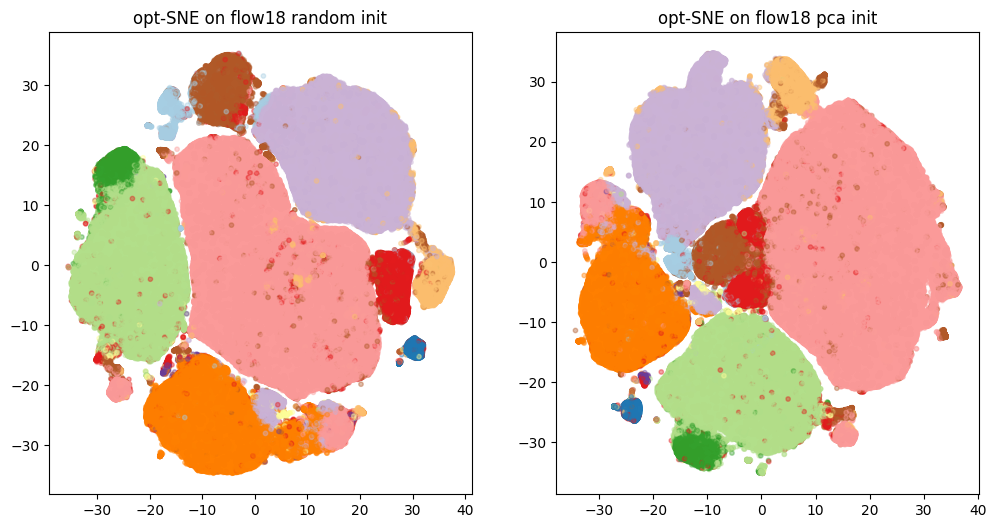
\includegraphics[width=\linewidth]{figures/pca_vs_random_init.png}
    \caption{PCA versus random initialization}
    \label{fig:PCA_vs_random}
\end{figure}
In our experiments, we do not necessarily see a visual improvement of the PCA initialized embedding over the random initialization one, but \textcolor{red}{one should look at other metrics to see how well the global structure is preserved e.g. Pearson correlation or Spearman correlation}. 

\subsection{Early Exaggeration}
Early exaggeration was first proposed as a method of optimizing t-SNE in \cite{vdMaa08}. They proposed multiplying all the $p_{ij}$ by a value $\alpha > 0$ for the first few iterations of the algorithm. Since our loss function encourages the $q_{ij}$ to model the $p_{ij}$ as closely as possible, we achieve artificially large $q_{ij}$ values this way. This means that relatively tight clusters are being formed, which can then move around more easily in space, making it easier to find a good global organization of the clusters. 

Open question: What should $\alpha$ be and for how many iterations should we keep EE on? 
\begin{itemize}
    \item \cite{vdMaa08} originally proposed $\alpha = 4$, for $50$ iterations out of $1000$ in total 
\end{itemize}

We can also understand early exaggeration from a dynamical systems viewpoint. 
We start by recalling the gradient of the t-SNE cost function: 
\begin{equation}
    \frac{\partial C}{\partial y_i} = 4 \sum_{j \neq i} (p_{ij} - q_{ij}) q_{ij} Z (y_i - y_j)
\end{equation}
with normalization term $Z = \sum_{k \neq l} (1+ \norm{y_k - y_l}^2 )^{-1}$. Notice that we can split the gradient into two parts 
\begin{equation}
    \frac{\partial C}{\partial y_i} = 4 (F_{\text{attr}} + F_{\text{rep}}) = 4 \left( \sum_{j \neq i } p_{ij} q_{ij} Z (y_i - y_j) - \sum_{j \neq i} q_{ij}^2 Z (y_i - y_j) \right) 
\end{equation}
where $F_{\text{attr}}$ denotes the sum of all attractive forces and $F_{\text{rep}}$ the sum of all repulsive forces. 

This next explanation is taken from \cite{LinStei22}.

Why does it make sense to call these attractive and repulsive forces? Since we want to minimize the cost function, we perform gradient descent and step in the direction of the negative gradient, so we consider the term
\begin{equation}
   - \frac{1}{4} \frac{\partial C}{\partial y_i} = \sum_{j \neq i } p_{ij} q_{ij} Z (y_j - y_i) - \sum_{j \neq i} q_{ij}^2 Z (y_j - y_i).  
\end{equation}
The first term is considered the attractive term, since it moves the point $y_i$ towards a weighted average of the other $y_i$. 
The weights $p_{ij} q_{ij} Z$ are bigger if the two points are close to each other (both in the low- and high-dimensional space). 
The second term has the opposite sign and thus pushes $y_i$ away from a weighted average of the other points. This time, however, the weights only depend on the closeness of points in the low-dimensional space. 
Put together, this means that the attractive term attracts points that are actually meant to be with each other (based on their similarity in the high-dimensional space) and the repulsive term pushes points apart that get too close in the embedding space, regardless of their real similarity. 

Early exaggeration has also been studied in detail empirically. \cite{BoehmBerens22} showed that stronger attractive forces (through high $\alpha$ values for EE) results in a better representation of continuous manifold structures while stronger repulsive forces (smaller $\alpha$ or no exaggeration) lead to a better recovery of discrete cluster structure. 

